\section{Experiments}\label{sec:experiments}
In this section, we describe the experiments conducted to evaluate the performance of the symbolic implementation of the Baum-Welch algorithm in the CuPAAL library by comparing it to the recursive implementation in Jajapy. The evaluation is based on two key aspects: execution time and accuracy.

We conduct two experiments:
\begin{itemize}
    \item \textbf{Performance Comparison} - Measuring runtime and accuracy across different models.
    \item \textbf{Scalability Analysis} - Evaluating performance as the number of states increases.
\end{itemize}

Through these experiments, we aim to answer the following research questions:
\begin{itemize}
    \item \textbf{Question 1}: How does the symbolic implementation of the Baum-Welch algorithm in CuPAAL compare to the recursive implementation in Jajapy in terms of runtime and accuracy?
    \item \textbf{Question 2}: How does the performance of the CuPAAL implementation scale with the size of the model?
\end{itemize}

\subsection{Experimental Setup}
All experiments are conducted using a set of \glspl{dtmc} and \glspl{ctmc} obtained from publicly available benchmarks~\cite{hartmanns2019quantitative}
\footnote{The models are available at \url{https://qcomp.org/benchmarks/}. The models are Leader\_sync, Brp, Crowds, Mapk, Cluster, and Embedded.}~\cite{hartmanns2019quantitative}.

Each experiment is run ten times.
We report the average runtime (full run and per iteration), the average number of iterations, log-likelihood per iteration, and the type of error based on the model type.

Experiments stop when reaching a convergence threshold of 0.05 (the Jajapy default) or a 4-hour runtime limit. The final iteration's results are recorded.

The training data is randomly generated based on these models, consisting of 30 observation sequences of length 10 for each model.

The implementations used are:
\begin{enumerate}
    \item The original Jajapy implementation.
    \item The symbolic CuPAAL implementation.
\end{enumerate}

\subsection{Experiment 1: Performance Comparison of Implementations}
The first experiment is based on the ideas from the experiment conducted in~\cite{reynouard2024learning}.

We split this experiment into two separate analyses: one focusing on \glspl{dtmc} and another on \glspl{ctmc}. Since \glspl{dtmc} estimate probabilities while \glspl{ctmc} estimate rates, we use different error measures for accuracy evaluation.

The experiments evaluate the efficiency and accuracy of the symbolic approach (CuPAAL) versus the recursive approach (Jajapy). We measure:
\begin{itemize}
    \item \textbf{Runtime Efficiency} - The average time per run.
    \item \textbf{Convergence Speed} - The average number of iterations required.
    \item \textbf{Accuracy} - Measured using log-likelihood and an average error.
\end{itemize}

\textbf{Log-likelihood:} Measures how well a learned model explains observed data.
For a given observation sequence $O$ and model $M$, it is defined as:
\begin{equation}
    \begin{aligned}
        \log P(O \mid M) = \sum_{t=1}^{T} \log P(O_t \mid M)
    \end{aligned}
\end{equation}
where $P(O_t|M)$ is the probability of observing $O_t$ given the model.

For both experiments on \glspl{dtmc} and \glspl{ctmc}, we expect the CuPAAL implementation to be faster than the Jajapy implementation due to the symbolic approach, which can avoid redundant calculations.
We also expect the accuracy to be consistent whether the type of model is a \gls{dtmc} or a \gls{ctmc} between the two implementations since the Baum-Welch algorithm is deterministic.

The results will be presented in tables for each model, showing the average time per run for each implementation, average number of iterations and log-likelihood and error for each model.

\subsubsection{Experiment 1A: Performance Comparison for DTMCs}
For \glspl{dtmc}, the models used are shown in \autoref{tab:dtmc_models}.
For \glspl{dtmc}, we use the absolute error as the measure of accuracy, because in \glspl{dtmc} we are estimating probabilities, and we are interested in the absolute difference between the real value and the estimated value.

The absolute error is calculated as follows:
\begin{equation}
    \begin{aligned}
        \text{Absolute Error} = |r - e|
    \end{aligned}
\end{equation}
where $r$ is the real value and $e$ is the expected value.

The results are presented for \glspl{dtmc} in \autoref{tab:leader_results}, \autoref{tab:brp_results}, and \autoref{tab:crowds_results}.

\subsubsection{Experiment 1B: Performance Comparison for CTMCs}
For \glspl{ctmc}, the models used are shown in \autoref{tab:ctmc_models}.

For \glspl{ctmc}, we use relative error as the measure of accuracy, since rates in CTMCs can vary significantly in magnitude, an absolute difference may not properly reflect the accuracy.
For example, a difference of 0.1 in a transition rate of 0.2 is a large error, whereas the same difference in a rate of 10 is negligible.
Using relative error ensures that errors are proportional to the expected value.

The relative error is calculated as follows:
\begin{equation}
    \begin{aligned}
        \text{Relative Error} = \cfrac{|r - e|}{e}
    \end{aligned}
\end{equation}
where $r$ is the real value and $e$ is the expected value.

The results are shown in \autoref{tab:mapk_results}, \autoref{tab:cluster_results}, and \autoref{tab:embedded_results}.

\begin{table}[!htb]
    \centering
    \caption{DTMC models}
    \label{tab:dtmc_models}
    \begin{tabular}{ll}
        \toprule
        Name         & Number of States \\
        \midrule
        Leader\_sync & 274              \\
        %Oscillators  & 453              \\
        Brp          & 886              \\
        Crowds       & 1145             \\
        \bottomrule
    \end{tabular}
\end{table}

\begin{table}[!htb]
    \centering
    \caption{CTMC models}
    \label{tab:ctmc_models}
    \begin{tabular}{lll}
        \toprule
        Name     & Number of States \\
        \midrule
        Mapk     & 118              \\
        Cluster  & 820              \\
        Embedded & 3480             \\
        \bottomrule
    \end{tabular}
\end{table}


\begin{table}[!htb]
    \centering
    \caption{Leader\_sync results}
    \label{tab:leader_results}
    \begin{tabular}{lllll}
        \toprule
        Implementation & Iter & Time(s) & Avg $\delta$ & Log-likelihood \\
        \midrule
        Jajapy         & 0    & 0       & 0            & 0              \\
        CuPAAL         & 0    & 0       & 0            & 0              \\
        \bottomrule
    \end{tabular}
\end{table}

\begin{table}[!htb]
    \centering
    \caption{Brp results}
    \label{tab:brp_results}
    \begin{tabular}{lllll}
        \toprule
        implementation & Iter & Time(s) & avg $\delta$ & log-likelihood \\
        \midrule
        Jajapy         & 0    & 0       & 0            & 0              \\
        CuPAAL         & 0    & 0       & 0            & 0              \\
        \bottomrule
    \end{tabular}
\end{table}

\begin{table}[!htb]
    \centering
    \caption{Crowds results}
    \label{tab:crowds_results}
    \begin{tabular}{lllll}
        \toprule
        implementation & Iter & Time(s) & avg $\delta$ & log-likelihood \\
        \midrule
        Jajapy         & 0    & 0       & 0            & 0              \\
        CuPAAL         & 0    & 0       & 0            & 0              \\
        \bottomrule
    \end{tabular}
\end{table}

\begin{table}[!htb]
    \centering
    \caption{Mapk results}
    \label{tab:mapk_results}
    \begin{tabular}{lllll}
        \toprule
        implementation & Iter & Time(s) & avg $\delta$ & log-likelihood \\
        \midrule
        Jajapy         & 0    & 0       & 0            & 0              \\
        CuPAAL         & 0    & 0       & 0            & 0              \\
        \bottomrule
    \end{tabular}
\end{table}

\begin{table}[!htb]
    \centering
    \caption{Cluster results}
    \label{tab:cluster_results}
    \begin{tabular}{lllll}
        \toprule
        implementation & Iter & Time(s) & avg $\delta$ & log-likelihood \\
        \midrule
        Jajapy         & 0    & 0       & 0            & 0              \\
        CuPAAL         & 0    & 0       & 0            & 0              \\
        \bottomrule
    \end{tabular}
\end{table}

\begin{table}[!htb]
    \centering
    \caption{Embedded results}
    \label{tab:embedded_results}
    \begin{tabular}{lllll}
        \toprule
        implementation & Iter & Time(s) & avg $\delta$ & log-likelihood \\
        \midrule
        Jajapy         & 0    & 0       & 0            & 0              \\
        CuPAAL         & 0    & 0       & 0            & 0              \\
        \bottomrule
    \end{tabular}
\end{table}

\subsection{Scalability Experiment}
The primary objective of this experiment is to evaluate the scalability of the proposed symbolic implementation of the Baum-Welch algorithm in comparison to the recursive implementation in Jajapy.
Specifically, we aim to measure the time required to learn \glspl{dtmc} and \glspl{ctmc} over the number of states.
We measure:
\begin{itemize}
    \item \textbf{Runtime efficiency} - The average time per run.
\end{itemize}

For this experiment, we selected two models-\textit{leader\_sync} (\gls{dtmc}) and \textit{polling} (\gls{ctmc})—as they represent those used in the performance comparison experiment and scale well to large state spaces.

\subsubsection{Experiment 2A: Scalability for DTMCs}
In this experiment, we evaluate the scalability of CuPAAL for \glspl{dtmc} by measuring runtime efficiency as the number of states increases.
We use the \textit{leader\_sync} model, scaling from 26 to 1050 states.

This experiment provides insights into how the symbolic approach scales as model complexity increases.
The results are shown in \autoref{fig:leader_results}.
We expect CuPAAL to demonstrate lower runtime and improved scalability, while maintaining accuracy comparable to Jajapy.

\begin{figure}
    \centering
    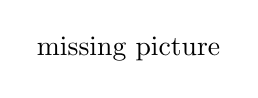
\begin{tikzpicture}
        \node {missing picture};
    \end{tikzpicture}
    \caption{Scalability results for the leader\_sync model}
    \label{fig:leader_results}
\end{figure}

\subsubsection{Experiment 2B: Scalability for CTMCs}
In this experiment, we evaluate the scalability of CuPAAL for \glspl{ctmc} by measuring runtime efficiency as the number of states increases.
We use the \textit{polling} model, scaling from 36 to 1334 states.

This experiment provides insights into how the symbolic approach scales as model complexity increases.
The results are shown in \autoref{fig:polling_results}.
We expect CuPAAL to demonstrate lower runtime and improved scalability, while maintaining accuracy comparable to Jajapy.

\begin{figure}
    \centering
    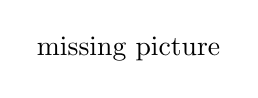
\begin{tikzpicture}
        \node {missing picture};
    \end{tikzpicture}
    \caption{Scalability results for the polling model}
    \label{fig:polling_results}
\end{figure}
